\chapter{Technological Foundation (11)}
\label{chap:technological-foundation}
\epigraph{I became convinced from the start that the notion of a state and a transition to a new state was fundamental to their thinking about the system.}{\textit{David Harel}}
Crossing the interdisciplinary boundaries between programming and psychology needs the definition of the technical concepts that are referenced.
For example knowing what is meant by \emph{state} and \emph{transition} in David Harel's psychological discovery is necessary to understand why this might impact the way people think about systems. 
As stated by \textcite{schraube_ich_2012} the interaction between a person's psyche and technology is always bidirectional, we get shaped by technology the same way we shape it.

\section{Characteristics of Software Development Processes}
\label{sec:characteristics-of-software-development-processes}
Upon answering the question on how communication in software development processes could be improved using technology, it's important to define those, take a quick look at the history and examine the difficulties of changing requirements.

Independent of the model used in software development six main phases can be identified, namely: \emph{requirements analysis}, \emph{specification}, \emph{design}, \emph{implementation}, \emph{testing} and \emph{maintenance} \autocite{harel_statecharts:_1987}.
Based on those phases there emerged a number of different software development models which can be subdivided into four ways of procedure: \emph{sequential}, \emph{incremental}, \emph{iterative} and \emph{iterative-incremental} \autocite{mayr_projekt_2005}.
Based on the historical events those can be divided into traditional paradigms of software development and modern paradigms of software development, where the latter mainly includes the iterative-incremental way of doing things.
The following overview is summarized and translated mainly on the information provided in \autocite{mayr_projekt_2005}.

\subsection{Traditional Paradigms}
\label{sub:traditional-software-development-paradigms}
The original reason for establishing paradigms in software development was making it planable, organizable and controllable.
Sequential models were introduced with the main idea that the previously described phases of software development could be completely separated and completed one after each other, starting the next one after the previous one was fully completed.
Problems arose from missing customer interaction and a long time to market, which led to the development of incremental paradigms.
In contrast to the sequential model software development was now seen as a gradual process that allowed validation, stepping back and re-implementation of only one single phase.
In 1970 Winston W. Royce introduced the Waterfall Model, which 
\todo{TODO}

- Developing Software does not happen Top-Down, but the conceptual models are closely related to the Waterfall Model \ref{sec:mental-models} \autocite[275]{kitchenham_research_1990}


- Strategic vs. Tactical Programming \autocite[13--18]{ousterhout_philosophy_2018}
- Bottom-Up-Approach \autocite[17]{horrocks_constructing_1999}
- Layered Behavioural Model (human centered) \autocite[254]{curtis_psychology_1990}
- Boundary Spanners \autocite[264]{curtis_psychology_1990}
- CITE: what makes the software development process special \autocite[274]{kitchenham_research_1990}
- "any documentation being an auxiliary, secondary product" \autocite{naur_programming_1985}
- Programming as a Social Activity \autocite{weinberg_psychology_1971}

\subsection{Modern Paradigms}
\todo{TODO}
\label{sub:modern-software-development-paradigms}
- On why agile can't work (\ref{sec:programming-as-theory-building}) \autocite[232--233]{naur_programming_1985}
\subsection{Requirements Engineering and Changing Requirements}
\todo{TODO}
- Requirements Specification \autocite[32]{leveson_experiences_1991}
- Information Loss \autocite[265]{curtis_psychology_1990}

\section{Statecharts}
\label{sec:statecharts}
Invented in 1983 by David Harel Statecharts are a "A Visual Formalism for Complex Systems".
While working on avionic systems for the Israeli Air Force David Harel was asked to help taming the complexity of reactive systems.
A reactive system is dominated by its "[...] reactivity; its event-driven, control-driven, event-response nature, often including strict time constraints, and often exhibiting a great deal of parallelism. A typical reactive system is not particularly data intensive or calculation intensive" \autocite{harel_statecharts_2007}.
Reading this pretty technical definition of a system Statecharts are aimed for one might question the relevance about Statecharts in software used by all of us at a daily basis.
Ian Horrocks provides an answer to this question by specifying the \emph{event-action paradigm} \autocite{horrocks_constructing_1999}.
User Interfaces are event-driven, they present screens with data and wait for some user interactions.
Based on those they react, thus fulfilling all the requirements for a reactive system.
And because every software that is interacted with has some kind of user interface, all those programs can utilize Statecharts as a way of handling state.

Describing a visual notation with words is contradictory, so let's take a look at \ref{fig:statecharts-example} taken out of the original paper \textcite{harel_statecharts:_1987}.
This Statechart describes part of the behaviour of a digital wrist watch.
The rounded rectangles describe states the system can be in and the labelled arrows between those describe the state transitions.
Basically a Statechart is an enhanced mixture between state diagrams and flow charts.
This also explains where the name comes from, according to \citeauthor{harel_statecharts_2007} the term \emph{Statecharts} was the only unused combination of "'state' or 'flow' with 'chart' and 'diagram'" in 1983.

\begin{figure}[h]
\centering
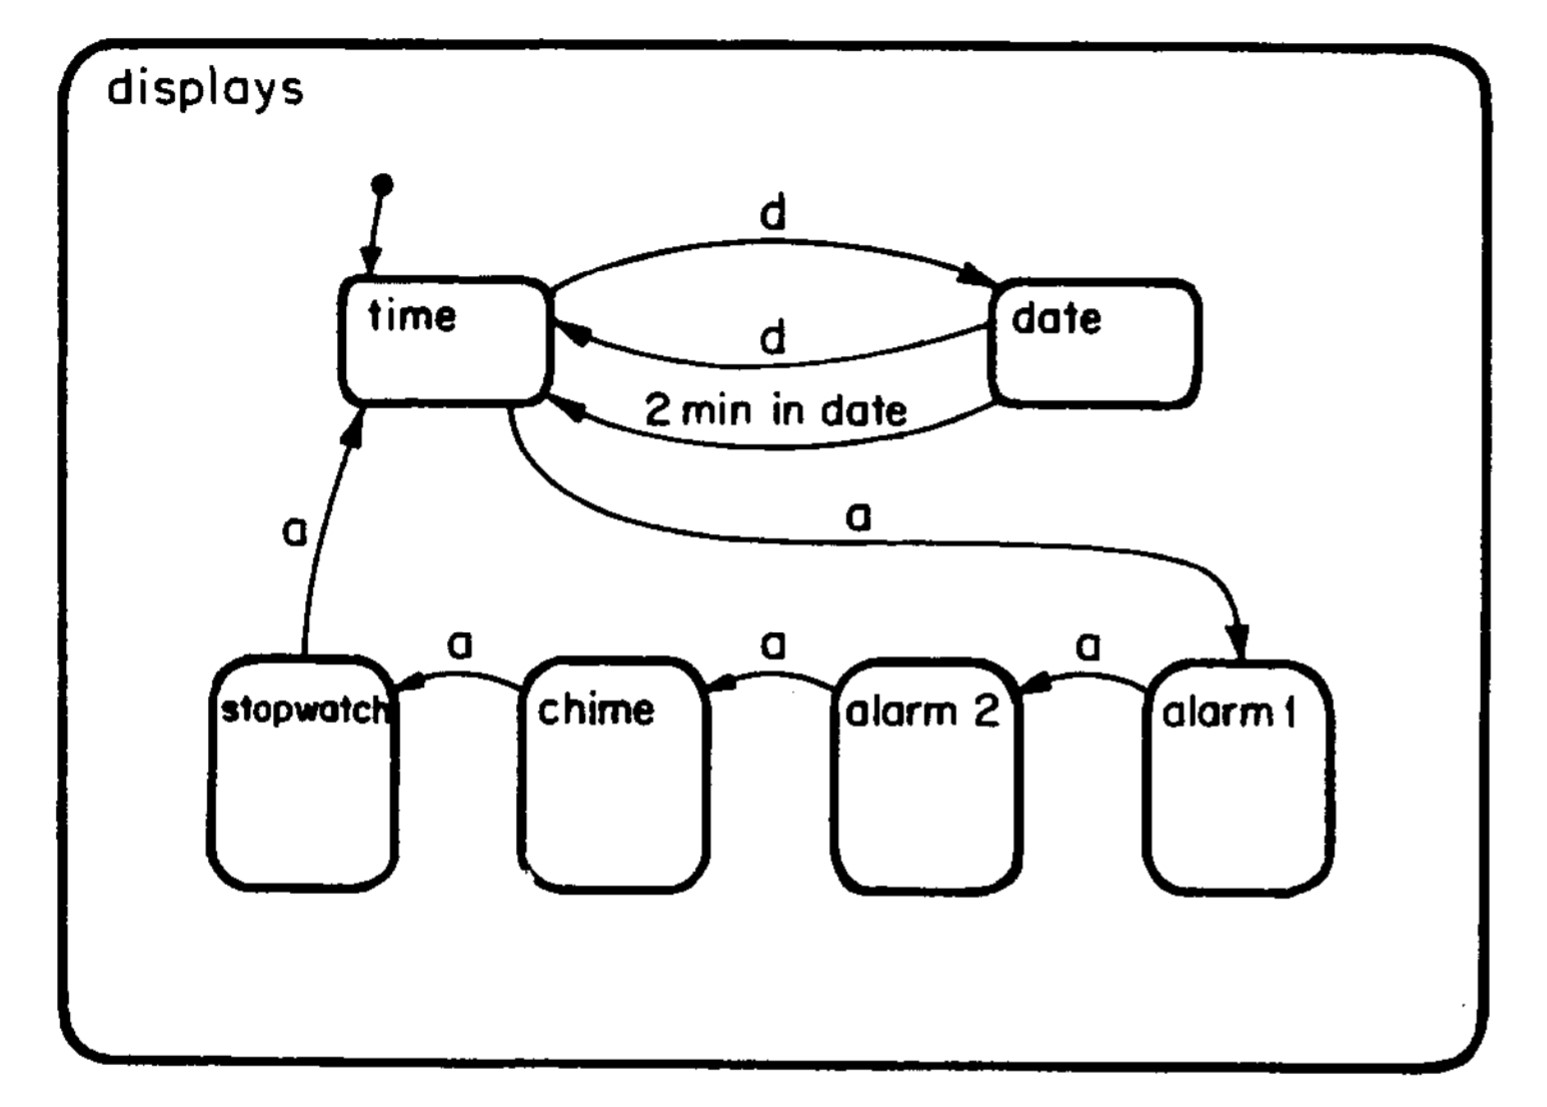
\includegraphics[width=0.8\textwidth]{small-statechart-example}
\caption{Example Statechart for a Digital Watch Interface}
\label{fig:statecharts-example}
\end{figure}

As T.G.R. Green defines in \textcite[3]{green_pictures_1982} "A \emph{program} is a succinct description of a temporal process."
Martin Glinz describes why Statecharts perfectly fit Green's definition of a program: "Naturally, statechart models will concentrate on requirements concerning dynamic system behavior and interaction" \autocite[1]{glinz_statecharts_2002}.
Taking a look at \cref{fig:statecharts-example} how does this Statechart transmit this information?
\begin{itemize}
    \item The outermost box \emph{displays} is a compound state containing multiple sub-states such as \emph{time}, \emph{data}, \emph{alarm 1} and so on. In Statecharts a compound state is defined by having multiple sub-states with exactly one being active at a certain point in time.
    \item The arrow originating in a black dot leading into \emph{time} specifies that this state is the initial active state of \emph{displays}.
    \item The arrows labeled \emph{d} between \emph{time} and \emph{date} can be translated to a toggle functionality between the time and display state of the watch.
    \item The arrow labeled with \emph{2 min in date} follows exactly its description. If the state \emph{date} was active for two minutes and no event occured the state \emph{time} is automatically entered.
    \item If the system is in state \emph{time} and the event \emph{a} occures it will transition to \emph{alarm 1}, on another press of \emph{a} into state \emph{alarm 2} and so on.
\end{itemize}

One of the most important properties of Statecharts in compared to source code as text is the visibility of valid and invalid transitions.
"Users" of the Statechart immediately conclude which events are possible in which state.
The reverse is also true and because the semantics of Statecharts are defined in a way that only events that are allowed in the current state lead enable transitions, programs are more robust and less faulty \autocite{horrocks_constructing_1999}.
For a full overview of the available features of Statecharts please refer to \textcite{harel_statecharts:_1987}.

\subsection{The Goals Behind}
\label{sub:goals-behind-statecharts}
In \citeyear{harel_statecharts_2007} David Harel published his personal story behind Statecharts titled "Statecharts in the Making: A Personal Account" \autocite{harel_statecharts_2007}.
In this paper he talks about his psychological ideas and observations during the development of Statecharts in the eighties.
Apart from creating a \emph{visual formalism} for reactive systems, he wanted to create a notation for \emph{model-based development} (which became really popular with the UML [\textcite{cook_unified_2017}]) and create an executable model where the behaviour "can and should be executed just like conventional computer programs [...]" \autocite[1]{harel_statecharts_2007}.
This technical goals lay the foundation for two of his goals that can be attributed to social psychology \autocite[3--4]{harel_statecharts_2007}:
\begin{enumerate}
    \item "The goal was to try to find, or to invent for these experts, a means for simply saying what they seemed to have had in their minds anyway."
    \item "The goal was to find a way to help take the information that was present collectively in their heads and put it on paper, so to speak, in a fashion that was both well organized and accurate."
\end{enumerate}

The above mentioned \emph{executability} of Statecharts is another fundamental of David Harel's ideas \autocite[7]{harel_modeling_1998}.
Back in the eighties executable models weren't the standard, but this simulation aspect takes a lot of cognitive load off the developer.
Back then when Statecharts were introduced the graphics and input capabilities of computers were uncomparable to those used today, but even then David Harel imagined "[...] graphical workstations with large (blackboard size?) displays of fantastic resolution [...]" \autocite[272]{harel_statecharts:_1987}.
More than 30 years later devices like the Microsoft Surface Hub\footnote{\url{https://www.microsoft.com/en-us/surface/business/surface-hub-2}} exist, that perfectly match this description.
Combined with Bret Victor's ideas of instant code executability \autocite{victor_inventing_2012} this could be the perfect match for an interactive development environment based on Statecharts.

\subsection{Aligning Thoughts with Fractal Architectures}
\label{sub:aligning-thoughts-with-fractal-architectures}
Comparing different approaches to user interface development André Staltz coined the term \emph{fractal architecture} as "[an] architecture is said to be fractal if subcomponents are structured in the same way as the whole is" \autocite{staltz_unidirectional_2015}.
Fractals are a mathematical concept of geometric figures that appear the same at different levels.
The most common fractal figure is the Mandelbrot set \autocite{mandelbrot_fractal_1982}.

As described earlier Statecharts feature the concept of compound states, wherein states can be nested inside each other.
This property perfectly maps to "geometric figures that appear the same at different levels" and André Staltz's definition of fractal architectures.
This state nesting allows to refine the behaviour of a certain state by adding sub-states and thus adapting to new requirements without breaking others \autocite{harel_statecharts:_1987}.
\autocite{leveson_experiences_1991} discuss the two main strategies of transforming requirements into software: \emph{top-down} and \emph{bottom-up}.
The top-down strategy is based on top-down refinement where requirements are deconstructed one after one, starting from the most abstract one transitioning down the tree of requirements.
Unfortunately this process only works for experts possessing a huge knowledge in software design as well as the domain they have to solve the problem in.
The bottom-up strategy on the other hand is characterized by less upfront thoughts about design and immediately starting with the implementation of requirements at a very detailled level.
A major problem using this approach is that a well designed software architecture is nearly impossible to reach, especially as applications get larger \autocite{horrocks_constructing_1999}.
As stated in \autocite{leveson_experiences_1991} programmers constantly switch between those two strategies while developing software.

This is exactly the point where the fractal nature of Statecharts can be aligned to the characteristics of programming.
States itself can be nested as well as refined using sub-states, directly resembling the composition and decomposition of requirements as shown by \textcite{leveson_experiences_1991}.
\textcite{glinz_statecharts_2002} already started research in the direction of transforming requirements into Statecharts, but only from a technical and not from a psychological perspective.


\section{Hole Driven Development}
\label{sec:hole-driven-development}
The term \emph{Hole-Driven Development} is not yet scientifically defined, but based on other programming concepts like \emph{Type-Driven Development} \autocite{brady_type-driven_2017} or \emph{Test-Driven Development} \autocite{mccracken_digital_1957}.
The main idea stems from the Agda programming language\footnote{\url{https://wiki.portal.chalmers.se/agda/pmwiki.php}} where \emph{holes} were called \emph{goals}.
Apart from Agda, Haskell\footnote{\url{https://www.haskell.org/}} and Idris\footnote{\url{https://www.idris-lang.org/}} feature the concept of holes.
The common properties of those languages is their functional nature and a very sophisticated type system, those two things lay the foundation for Hole-Driven Development as currently understood.

Simply said a \emph{hole} declares a missing part in your application.
\textcite{gamari_haskell_2019} contains the most comprehensive description of the concept of holes, while \textcite{brady_type-driven_2017} created the following example.

\subsection{Example in Idris}
\label{sub:hole-driven-development-in-idris}
The Idris program in \ref{fig:idris-program-hole} demonstrates the simplest possible hole.
In line \verb|2| the function \verb|main| is defined that should print something (\verb|putStriLn|) to the console.
The "hole"-part of this program is \verb|?greeting|.
Signaling a hole, the questionmark tells the Idris compiler that something in this program is missing, that the developer didn't specify yet.
The syntax using a questionmark resembles a question to the compiler.

\begin{figure}[h!]
\begin{lstlisting}[language=Haskell,firstnumber=1]
main : IO ()
main = putStrLn ?greeting
\end{lstlisting}
\caption{A Hole in an Idris program}
\label{fig:idris-program-hole}
\end{figure}

Edwin Brady coined the phrase "the compiler as your lab-assistant" \autocite{brady_type-driven_2017}.
His imagination of a compiler is that of a counterpart you interact with or pair-program together.
You tell the compiler all the things that are currently in your mind and as a reward you can ask questions and the compiler will try to answer those based on the knowledge you already gave.
In terms of psychology this is a pretty humane way of interacting with the computer.

A practical example of this ideas looks like the following output of Idris' interactive command line interface.
Using \verb|:t greeting| you can ask the compiler for the type of the hole "greeting".
As an answer you get \verb|greeting : String| which tells you that you have to find some value that is of type String, or in non-technical types simply a text.

\begin{verbatim}
*Hello> :t greeting
--------------------------------------
greeting : String
\end{verbatim}

In contrast to the previous example if you just try to use \verb|greeting| the Idris compiler tells you that you have a hole in your program labelled \emph{greeting} of type String.
This shows the communication process Edwin Brady talks about.

\begin{verbatim}
*Hello> greeting
?greeting : String
\end{verbatim}

"Holes allow you to develop programs \emph{incrementally}, writing the parts you know and asking the machine to help you [...]" \autocite[21]{brady_type-driven_2017}.
Stepping a little bit back and comparing this way of developing software to how software development processes evolved (\cref{sub:modern-software-development-paradigms}) the similarities are unmistakable.
Let's take a look at how holes are simulated in programming languages that don't support this feature natively, before we get to psychological observations that were already discovered in the field of psychology of programming.

\subsection{Simulating Holes}
In languages that do not provide the feature of typed holes programmers tend to come up with alternative solutions to holes without knowing of their existence.
As seen in \cref{sub:incomplete-thoughts} indicates the process of creating these holes is natural, but the features of a programming language constrain the usefulness and direct mapping to the users mental model.
There are mainly two ways of simulating holes:
\begin{description}
\item[Exceptions] One might throw Exceptions as documented in \textcite{microsoft_notimplementedexception_2020} to signal that a feature is not yet implemented.
\item[Comments] The other common way of deferring development of a particular method or feature is to mark it with a comment starting with \verb|TODO:|. E.\,g. in C\#\footnote{\url{https://docs.microsoft.com/en-us/dotnet/csharp/}} this looks like \verb|// TODO: Load state from previously suspended application|. Programming environments are able to parse this information and provide an overview for all \emph{Todos} as shown in \textcite{hogensen_use_2019}.
\end{description}
This might sound like a good surrogate at first, so what are the differences to real holes?
\begin{itemize}
    \item The previously described interaction with the compiler is missing completely.
    \item By using exceptions the program crashes at run-time, which results in buggy software. Additionally there is no real overview for all the simulated holes. One has to do a text-based search for the exception name.
    \item Utilizing comments doesn't result in the program crashing, rather not adhering to the specifications without any note at run-time.
    \item Both approaches act like a "do-it-later"-approach, without actively reminding the developer at a later time.
\end{itemize}

\subsection{Incomplete Thoughts}
\label{sub:incomplete-thoughts}
In the \citeyear{visser_expert_1990} conducted meta-analysis \citetitle{visser_expert_1990} \citeauthor{visser_expert_1990} collected thinking processes and strategies of expert programmers \autocite{visser_expert_1990}.
Comparing breadth-first and depth-first design methodologies they found out that expert developers vary in their usage and most of the time combine both strategies.
One commonality was the observation that the developers under research were observed making "notes to themselves" \autocite[241]{visser_expert_1990}.
Experts usually excel at maintaining relevant information in memory, nevertheless this memory capacity is limited and working on one problem might relate to other problems until there is not enough capacity left and they start taking those notes.
They conclude that "[...] before introducing the constraints of actual programming languages, experts very often use a personal pseudo-code" \autocite[242]{visser_expert_1990}.

Combining this research it seems plausible that real holes enhanced with comments could lead to a programming language that lets developers specify the already thought-out ideas in executable source code while still letting them express their ideas in natural language with the advantage of the programming environment caring about your ideas.